\documentclass[nooutcomes]{ximera}
%% handout
%% space
%% newpage
%% numbers
%% nooutcomes

\usepackage{fullpage}
\newcommand{\RR}{\mathbb R}
\renewcommand{\d}{\,d}
\newcommand{\dd}[2][]{\frac{d #1}{d #2}}
\renewcommand{\l}{\ell}
\newcommand{\ddx}{\frac{d}{dx}}
\newcommand{\dfn}{\textbf}
\newcommand{\eval}[1]{\bigg[ #1 \bigg]}

\usepackage{multicol}

\renewenvironment{freeResponse}{
\ifhandout\setbox0\vbox\bgroup\else
\begin{trivlist}\item[\hskip \labelsep\bfseries Solution:\hspace{2ex}]
\fi}
{\ifhandout\egroup\else
\end{trivlist}
\fi} %% we can turn off input when making a master document

\title{Section 3.2 Working with Derivatives}  

\begin{document}
\begin{abstract}		\end{abstract}
\maketitle

%problem1
\begin{problem}
	
	\begin{enumerate}

    \item
   
      If $f'(2)$ exists, then
      \begin{enumerate}
        \item
          $\lim_{x \to 2} f(x)$ must exist, but $\lim_{x \to 2} f(x) \ne f(2)$

        \item
          $\lim_{x \to 2} f(x) = f(2)$.

        \item
          $\lim_{x \to 2} f(x) = f'(2)$

        \item
          $\lim_{x \to 2} f(x)$ need not exist.
      \end{enumerate}
      \begin{freeResponse}
        The correct answer is (ii):
        \begin{align*}
          \mbox{$f'(2)$ exists} &\iff \mbox{$f$ differentiable at $x = 2$}\\
                                &\implies \mbox{$f$ continuous at $x = 2$}\\
                                &\iff \lim_{x \to 2} f(x) = f(2)
        \end{align*}
      \end{freeResponse}


    \item

      Assuming that $\lim_{x \to 0} \frac{\sin x}{x} = 1$, we can conclude
      \begin{enumerate}
        \item
          $\frac{0}{0} = 1$
        \item
          the tangent line to $y = \sin x$ at $(0,0)$ has slope $1$.

        \item
          you can cancel the $x$'s.

        \item
          for all $x$ near $0$, $\sin x = x$.

        \item
          for all $x$ near $0$, $\sin x \approx x$.
      \end{enumerate}
      \begin{freeResponse}
        This problem has two correct answers: (ii) and (v).

        Statement (ii) is true:
        \begin{align*}
          f'(0) &= \lim_{h \to 0} \frac{\sin (h + 0) - \sin (0)}{h} \\
                &= \lim_{h \to 0} \frac{\sin (h)}{h} \\
                &= 1\\
          &\implies \mbox{slope of tangent line at $(0,0)$ is $1$}
        \end{align*}

        Statement (v) is true:
        When $x$ is near $0$ the tangent line $y = x$ is a good approximation to $f$.
      \end{freeResponse}

  \end{enumerate}

	
\end{problem}	
	
%problem 2

	
\begin{problem}
  Define the function $f$ by $f(x) = x^{1/3}$ and consider the graph of this function:
  \begin{image}
    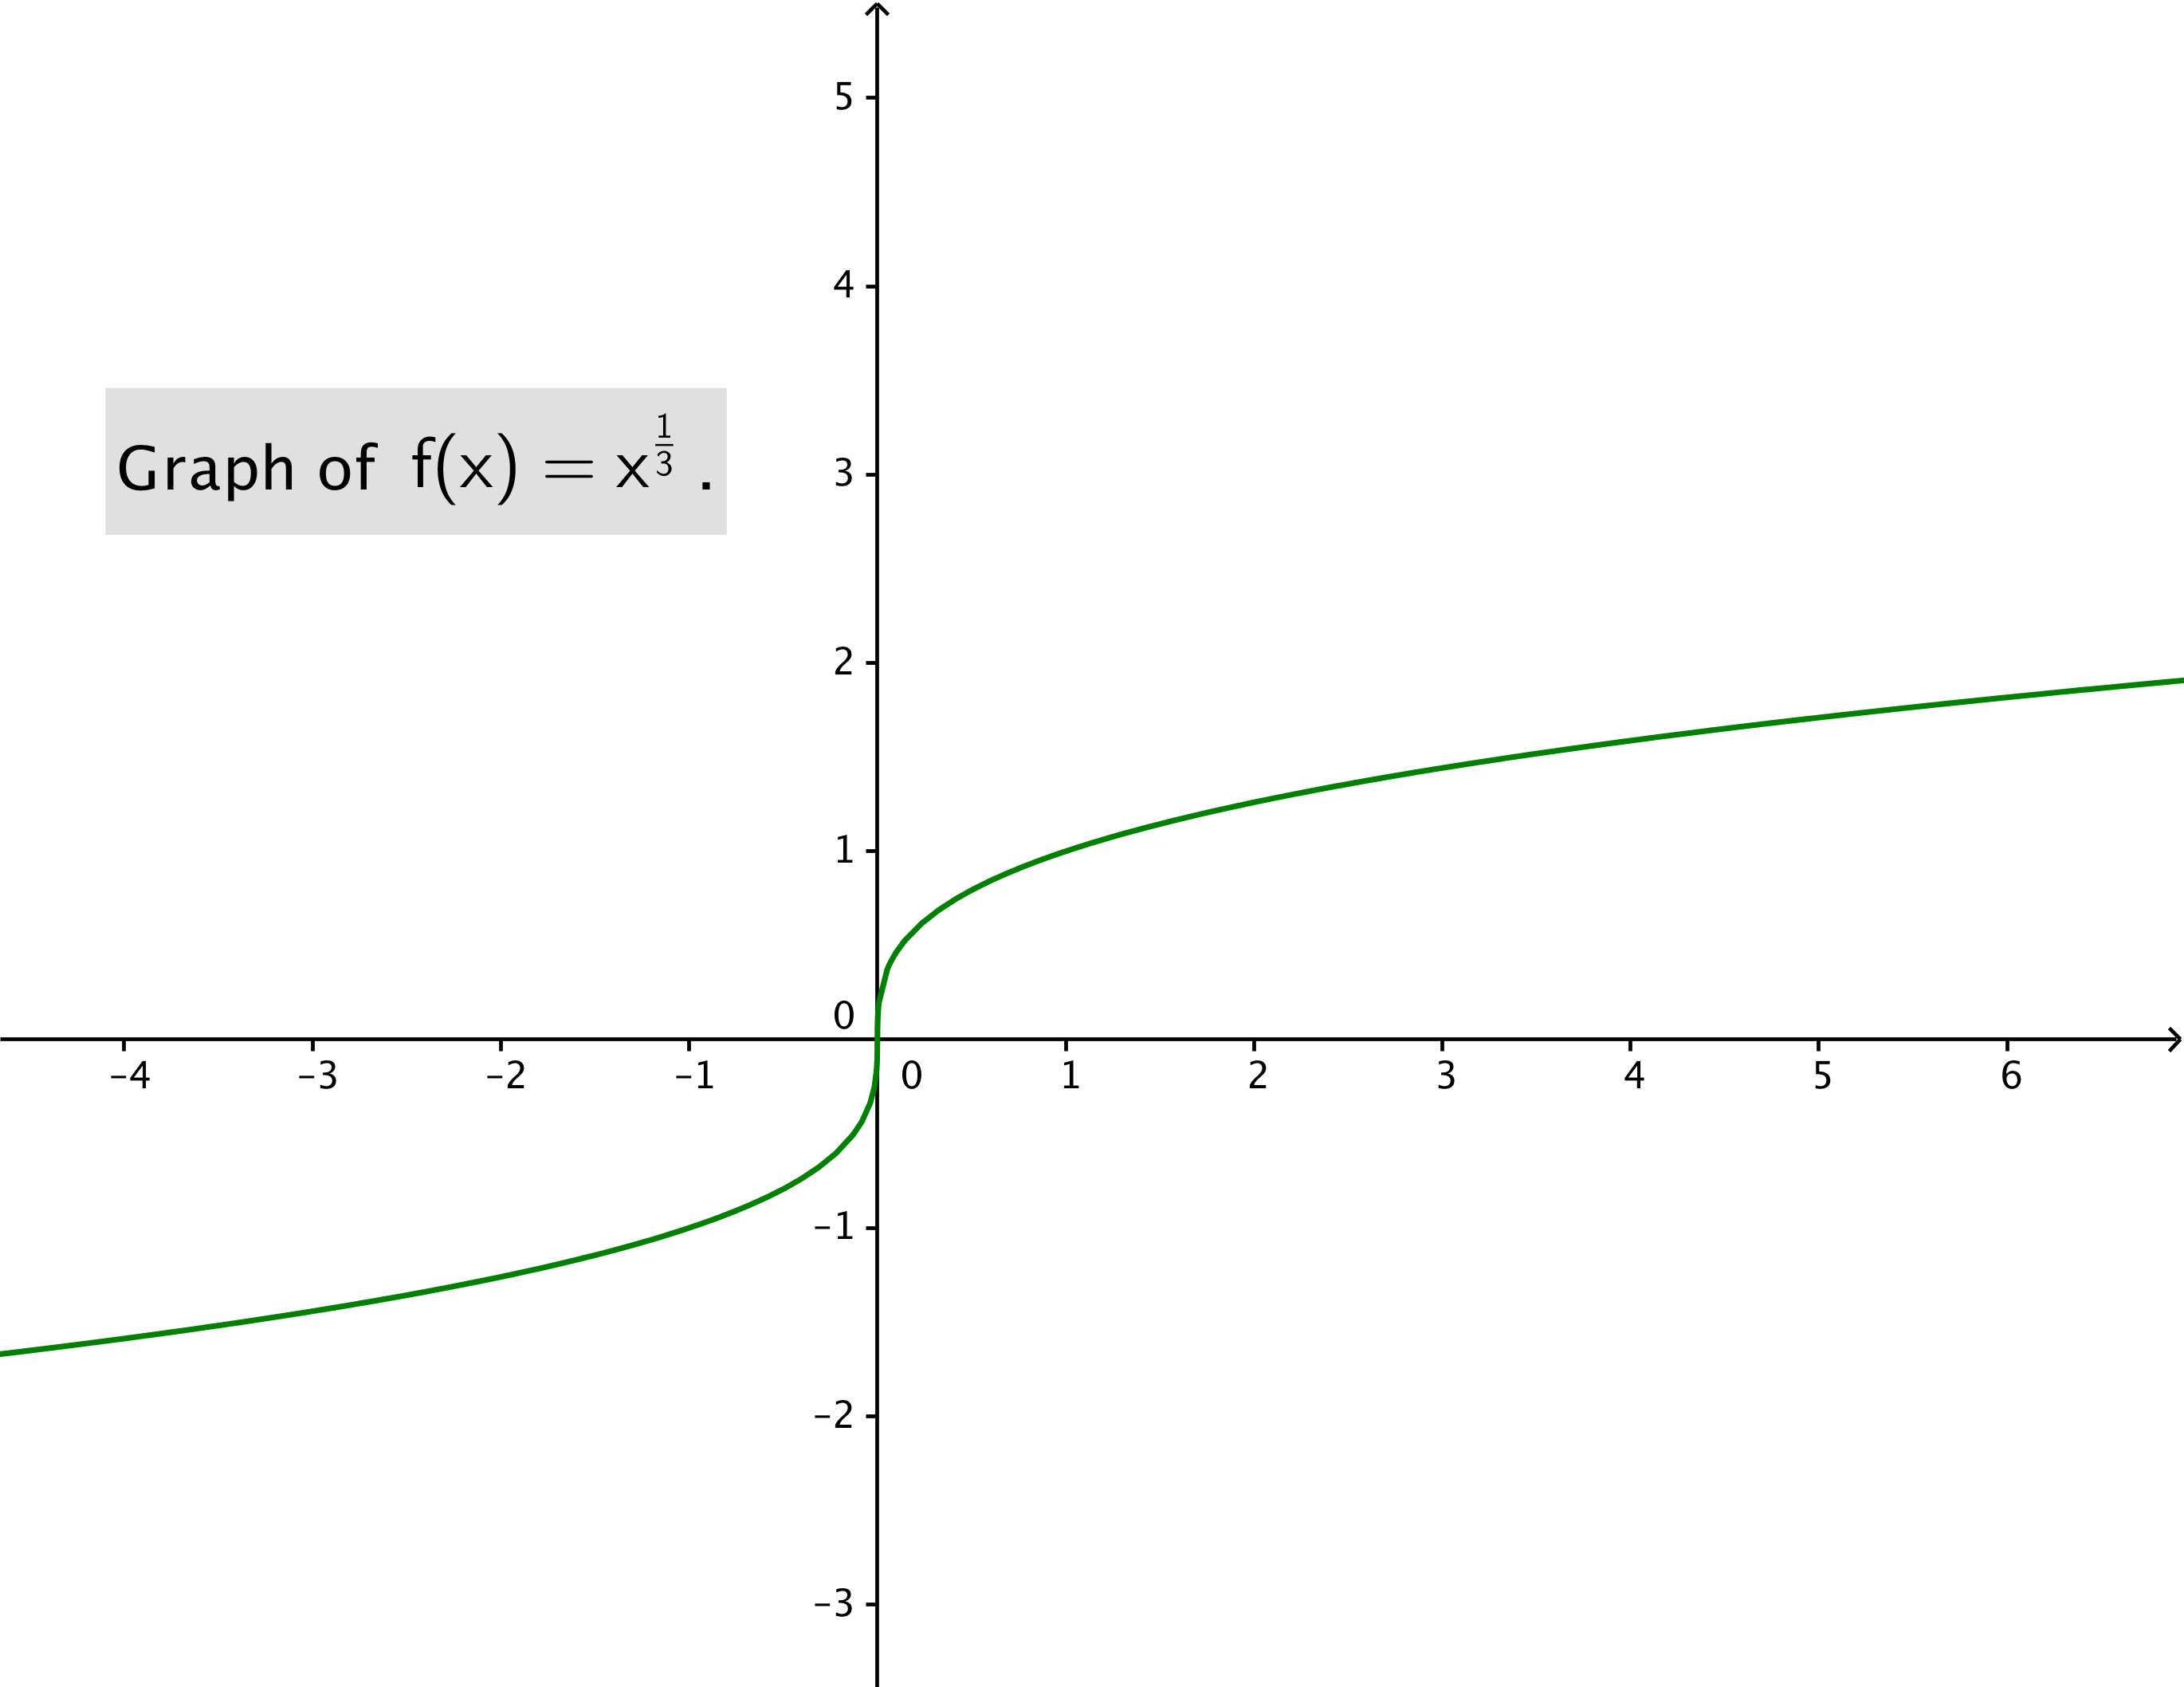
\includegraphics[scale = 0.4]{figure6.png}
  \end{image}

  Which of the following two statements are true:
  \begin{enumerate}
     \item The graph of $f$ has a tangent line at $x = 0$.
      \begin{freeResponse}
        This statement is \textbf{true}!
        The function $f$ has a vertical tangent at $x = 0$:
        \begin{image}
          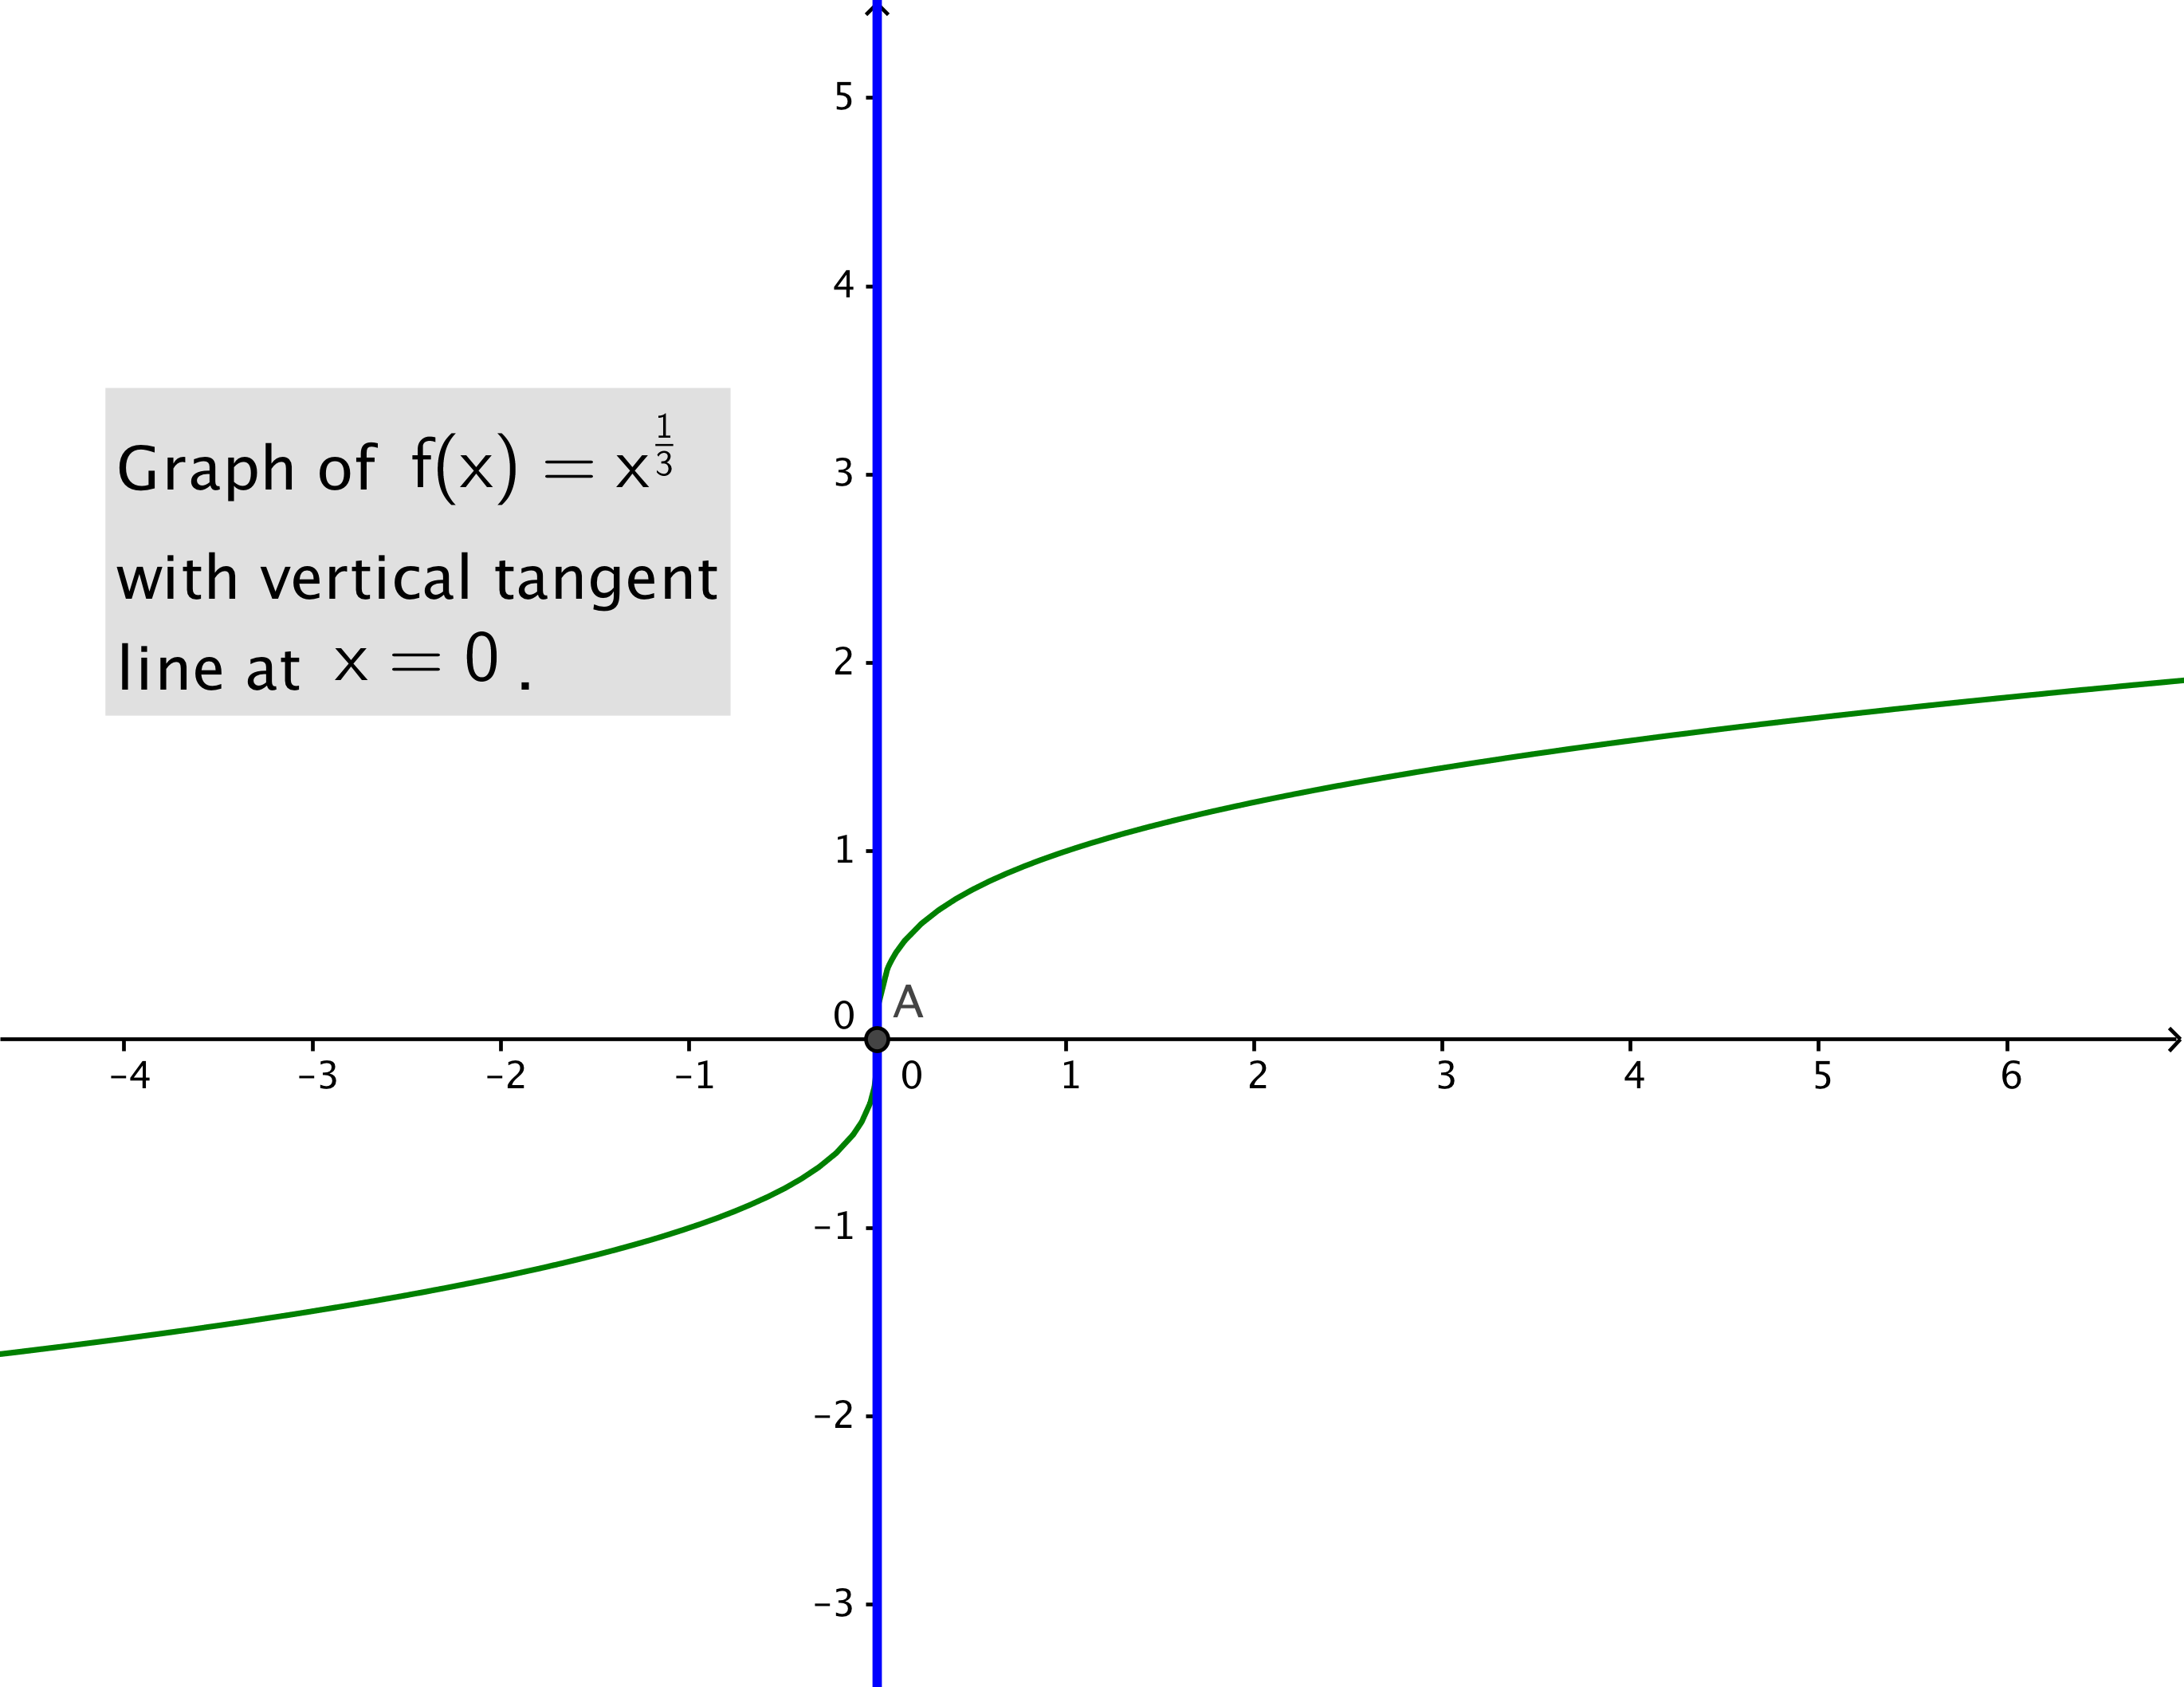
\includegraphics[scale = 0.4]{figure7.png}
        \end{image}
      \end{freeResponse}

    \item  The derivative $f'(0)$ is defined.
      \begin{freeResponse}
        This statement is \textbf{false}!
        \begin{align*}
          \lim_{h \to 0^+} \frac{f(0  + h) - f(0)}{h}
          &= \lim_{h \to 0^+} \frac{h^{1/3}}{h} \\
          &= \lim_{h \to 0^+} \frac{1}{h^{\frac{2}{3}}} \\	
          &= \infty\ \text{because the limit is of the form:}\ \frac{\text{pos}}{0^+}\\
          &\implies \mbox{$f'(0)$ is undefined}
        \end{align*}
      \end{freeResponse}
  \end{enumerate}
\end{problem}	
	
%problem 3		
\begin{problem}
  Suppose we are given the graph of a function $f$:
  \begin{image}
    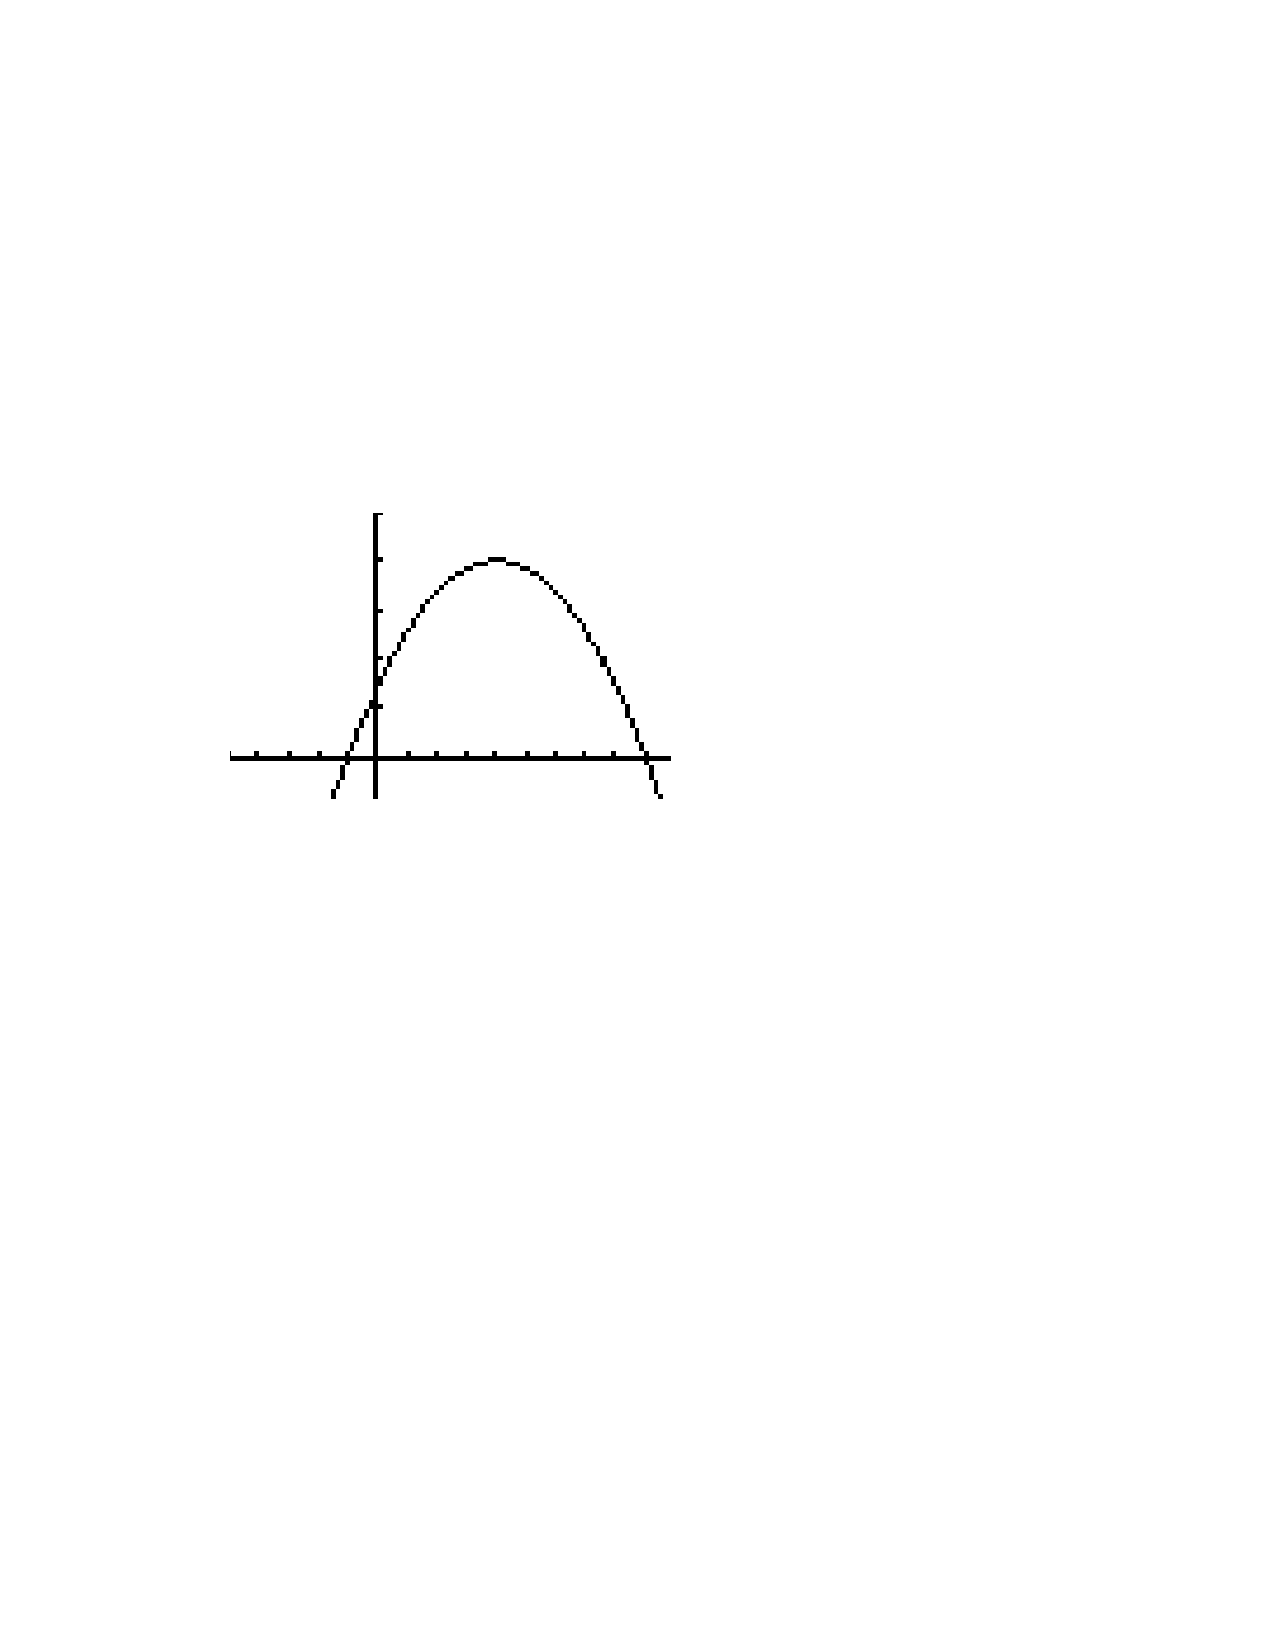
\includegraphics[scale=.7]{Figure1.png}
  \end{image}
  \begin{enumerate}
	%part a
    \item
      Use this graph to find the following:  (Assume all values will be integers or $+\infty$ or $-\infty$)
      \begin{enumerate}
        \item 
          all $x$ where $f(x) = 0$,
          \begin{freeResponse}
            $f(x)$ is zero when the function crosses the $x$-axis.
            Therefore $f(x) = 0$ when $x = -5, x=-1$, and $x = 5$.
          \end{freeResponse}

        \item 
          all $x$ where $f(x) > 0$, 
          \begin{freeResponse}
            $f(x)$ is positive when the graph of the function is above the $x$-axis.
            Therefore $f(x) > 0$ on $(-5,-1) \cup (5,\infty)$. 
          \end{freeResponse}

        \item
          all $x$ where $f(x) < 0$, and
          \begin{freeResponse}
            $f(x)$ is negative when the graph of the function is below the $x$-axis.
            Therefore $f(x) < 0$ on $(-\infty ,-5) \cup (-1,5)$.
          \end{freeResponse}

        \item
          all $x$ where $f(x)$ attains a local maximum and all $x$ where $f$ attains a local minimum.
          \begin{freeResponse}
            $f(x)$ has a local maximum at $x=-3$.
            $f(x)$ has a local minimum at $x=2$.
          \end{freeResponse}
      \end{enumerate}
	%part b
    \item

      Without sketching the graph of $f'$ find
      \begin{enumerate}
        \item 
          all $x$ where $f'(x) = 0$,
          \begin{freeResponse}
            $f'(x)$ is zero when the tangent line has a slope of zero, which is approximately at $x=-3$ and $x=2$.
            Note, for this question, these are the same answers as the (local) highest and lowest point for the graph of $f$.   
          \end{freeResponse}

        \item
          all $x$ where $f'(x) > 0$,
          \begin{freeResponse}
            ${f}'(x)$ is positive when the slope of the tangent line is positive.
            Observe that $f$ is increasing on $(-\infty ,-3), (2,\infty)$ and this same set of intervals is where the tangent lines have positive slope.
            Therefore $f'(x) > 0$ on $(-\infty ,-3), (2,\infty)$.
          \end{freeResponse}
        
        \item
          all $x$ where $f'(x) < 0$, and
          \begin{freeResponse}
            ${f}'(x)$ is negative when the slope of the tangent line is negative.
            Observe that $f$ is decreasing on $(-3,2)$ and this interval is where the tangent lines have negative slope.
            Therefore $f'(x) < 0$ on $(-3,2)$.
          \end{freeResponse}

        \item
          On the following intervals, does $f'(x)$ seem to be increasing or decreasing?
         
            \begin{enumerate}
		\item $(-\infty,0)$
			 \begin{freeResponse}
				decreasing
			  \end{freeResponse}
		\item $(0,\infty)$
			 \begin{freeResponse}
				increasing
			  \end{freeResponse}
	\end{enumerate}

      \end{enumerate}
	%part c
      \item
      Sketch a graph of $f'$.
      \begin{freeResponse}
        The graph of $f'$ is approximately
        \begin{image}
          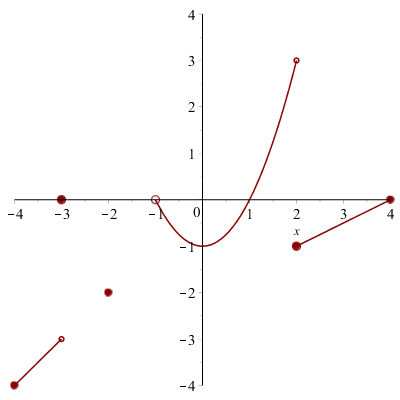
\includegraphics[scale = 0.5]{Figure2.png}
        \end{image}
      \end{freeResponse}
  \end{enumerate}
\end{problem}



%problem 4
\begin{problem}
  Use the graph of $g$
			\begin{image}
	 		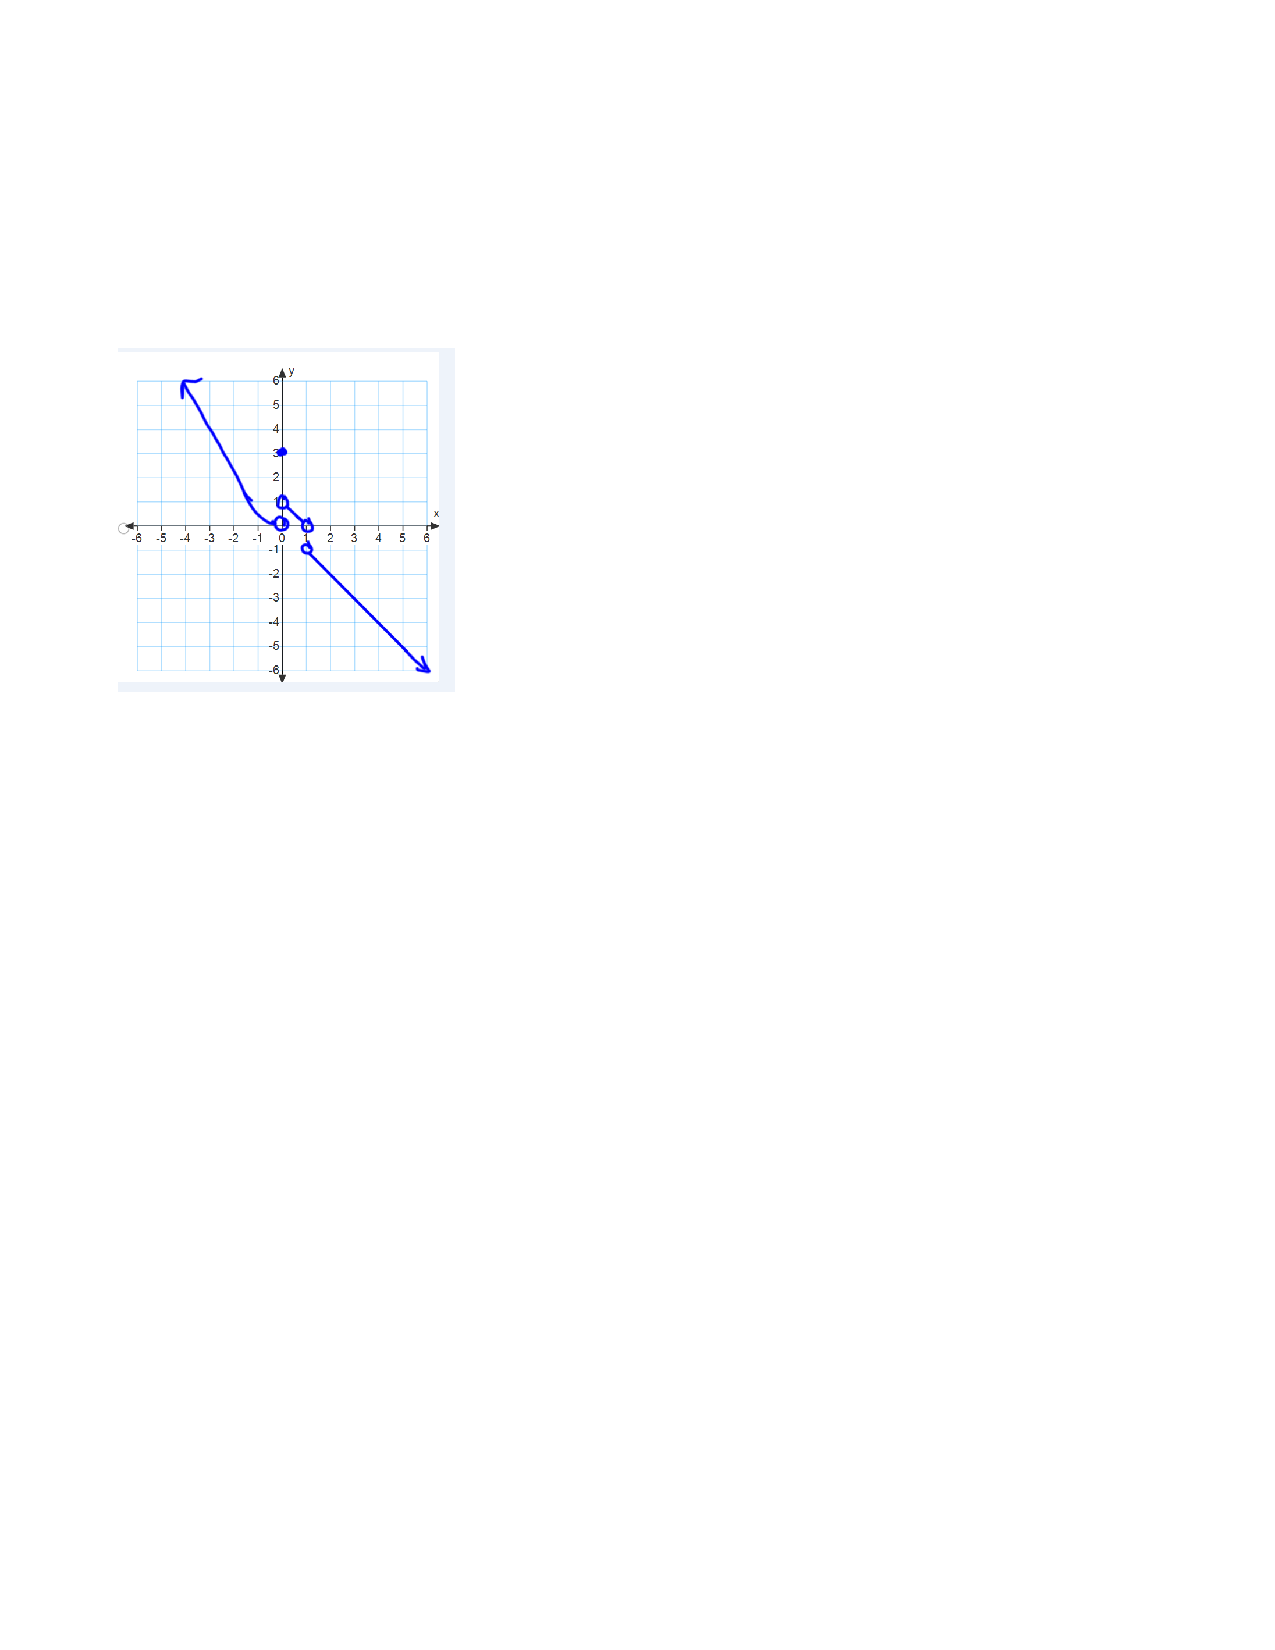
\includegraphics{Figure3.png}
			\end{image}
			

	\begin{enumerate}
	
	\item Find the values of $t$ in $(0,4)$ at which $g$ is not continuous.
		\begin{freeResponse}
		$g$ is not continuous at $t=1$.
		\end{freeResponse}
		
		
	
	\item Find the values of $t$ in $(0,4)$ at which $g$ is not differentiable.
		\begin{freeResponse}
		$g$ is not differentiable at $t=1$ and $t=2$.
		\end{freeResponse}
		
		\end{enumerate}



\end{problem}
	

%problem5
\begin{problem}

	 Given the following graph of a function $h$ sketch a graph of the derivative $h'$.
  \begin{image}
    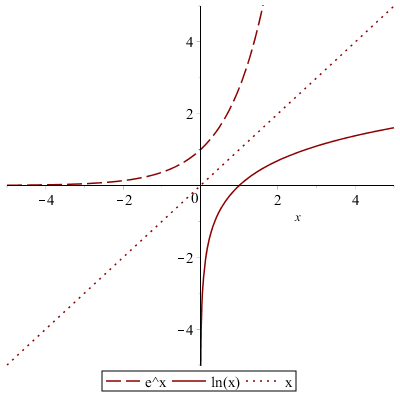
\includegraphics[scale=.7]{Figure4.png}
  \end{image}
  \begin{freeResponse}
    The graph of the derivative is in red.
    \textbf{Important Note:} Despite being drawn on the same graph, the ``units'' for $f$ and $f'$ are \emph{not} the same!
    \begin{image}
      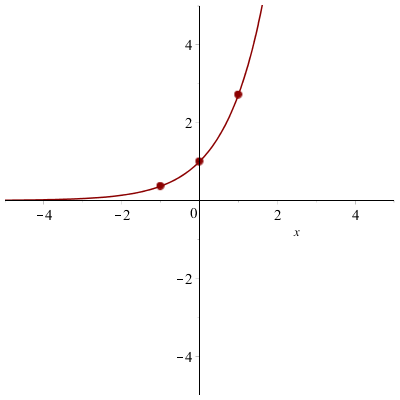
\includegraphics[scale = 0.7]{Figure5.png}
    \end{image}
  \end{freeResponse}
\end{problem}

%problem6
\begin{problem}
  \mbox{}
  \begin{enumerate}
    \item


      Fill in the blanks
      \[
        f'(x) = \lim_{\text{???}} \frac{\text{????}}{h}
      \]
      if the limit exists.
	\begin{freeResponse}
      \[
        f'(x) = \lim_{h \to 0} \frac{f(x + h) - f(x)}{h}
      \]
      if the limit exists.
	\end{freeResponse}
    \item
      Let 
      \[
        f(x) = \frac{1}{x + 4}.
      \]
      Use the (limit) \emph{definition} of derivative in (a) to find $f'(x)$.
      \begin{freeResponse}
        \begin{align*}
          f'(x) &= \lim_{h \to 0} \frac{f(x + h) - f(x)}{h} = \lim_{h \to 0} \frac{\frac{1}{x+h +4}-\frac{1}{x+4}}{h} \\
          &= \lim_{h \to 0} \frac{\frac{x+4 -(x+h +4)}{(x+h +4)(x+4)}}{h}\\
          &= \lim_{h \to 0} \frac{1}{h} \cdot \frac{-h}{(x+h +4)(x+4)} \\
          &= \lim_{h \to 0} \frac{-1}{(x+h +4)(x+4)} = \frac{-1}{(x+4)^2}
        \end{align*}
      \end{freeResponse}
  \end{enumerate}
\end{problem}

	
%problem7
\begin{problem}
Let $f(x) = |5-x|$.
	
	\begin{enumerate}
	
	%a
	\item For $a < 5$, find $f'(a)$.
	
		\begin{freeResponse}
		Recall that 
		$$f'(a) = \lim_{x \to a} \frac{f(x) - f(a)}{x-a}.$$
		When $a < 5$, $0 < 5-a$ and so $f(a) = |5-a| = 5-a$.  Since we are considering the limit as $x$ approaches $a$, (and therefore interested in values of $x$  really close to $a$), we may also assume that $x < 5$ and therefore $f(x) = 5-x$.  Thus
		\begin{align*}
		f'(a) &= \lim_{x \to a} \frac{f(x) - f(a)}{x-a}  \\
		&= \lim_{x \to a} \frac{(5-x) - (5-a)}{x-a}  \\
		&= \lim_{x \to a} \frac{-(x-a)}{x-a}  \\
		&= \lim_{x \to a} -1 = -1.
		\end{align*}

		\end{freeResponse}

	%b
	\item For $a > 5$, find $f'(a)$.
	
		\begin{freeResponse}
		When $a > 5$, $0 > 5-a$ and so $f(a) = |5-a| = -(5-a) = a-5$.  Since we are considering the limit as $x$ approaches $a$, we may also assume that $x > 5$ and therefore $f(x) = x-5$.  Thus
		\begin{align*}
		f'(a) &= \lim_{x \to a} \frac{f(x) - f(a)}{x-a}  \\
		&= \lim_{x \to a} \frac{(x-5) - (a-5)}{x-a}  \\
		&= \lim_{x \to a} \frac{x-a}{x-a}  \\
		&= \lim_{x \to a} 1 = 1.
		\end{align*}

		\end{freeResponse}
	%c
	\item Determine whether $f'(5)$ exists.  
	
		\begin{freeResponse}
		If  $f'(5)$ exists then $\lim_{x \to 5} \frac{f(x) - f(5)}{x-5}$ exists.  But when $x$ is close to $5$ it may be that $x>5$ or $x<5$.   So in order to find this limit, we have to check whether the two one-sided limits are equal.\\
		This means,  $\lim_{x \to 5^-} \frac{f(x) - f(5)}{x-5}=\lim_{x \to 5^+} \frac{f(x) - f(5)}{x-5}$\\ 


		\begin{align*}
		\lim_{x \to 5^-} \frac{f(x) - f(5)}{x-5}&=\lim_{x \to 5^-} \frac{-(x-5) - (0)}{x-5}=-1\\
		\lim_{x \to 5^+} \frac{f(x) - f(5)}{x-5}&=\lim_{x \to 5^+} \frac{(x-5) - (0)}{x-5}=1\\
		\lim_{x \to 5^-} \frac{f(x) - f(5)}{x-5} &\ne\lim_{x \to 5^+} \frac{f(x) - f(5)}{x-5}
		\end{align*}
		Therefore, $f'(5)$ does not exist.\\\\
			$f'(a) =   \left\{ \begin{array}{cl}
	1	 	&	\qquad \text{if } a>5					\\ \\
	\text{undefined}	&	\qquad \text{if } a=5	\\ \\
	-1			&	\qquad \text{if } a<5				\end{array} \right.  $
		\end{freeResponse}
		
	\item Sketch a graph of the function $f(x)$ and its derivative $f'(x)$

		\begin{freeResponse} \hfil
\begin{image}
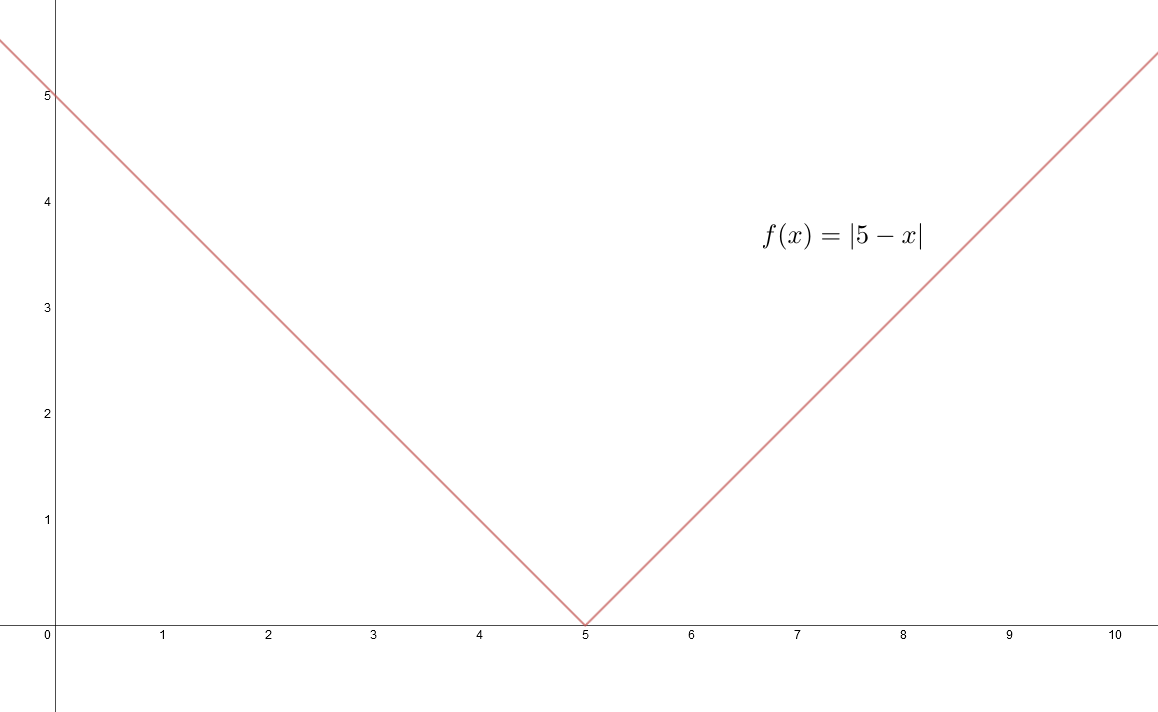
\includegraphics[scale = .3]{Figure12.png}
\end{image} 
\begin{image}
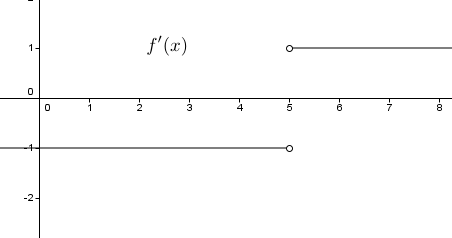
\includegraphics[scale = .9]{Figure13.png}
\end{image} 
		\end{freeResponse}

	\end{enumerate}


\end{problem}	
	
	


\end{document} 


















